%%% opt-ex1.png
\documentclass[border=1mm,10pt]{standalone}
\usepackage[utf8]{inputenc}
\usepackage{tikz}
\usetikzlibrary{calc}
\usetikzlibrary{shapes.geometric}

\begin{document}
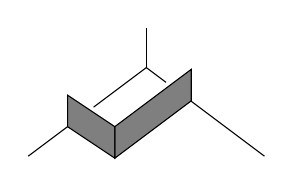
\begin{tikzpicture}

% walls
\draw (-1.5, -1.5*0.75) -- (-1, -0.75);
\draw (-0.67, -0.67*0.75) -- (0, 0) -- (0.25, -0.25*0.75);
\draw (0.57, -0.57*0.75) -- (1.5, -1.5*0.75);
\draw (0, 0) -- (0, 0.5);

% strips
\def\h{0.4}
\draw [fill=black, fill opacity=0.5]
    (-1, -0.75) -- ++(0, \h) -- ++(0.6, -0.4) -- ++(0, -\h) coordinate (B) -- cycle;
\draw [fill=black, fill opacity=0.5]
    (B) -- ++(0, \h) -- ++ (0.97, 0.97*0.75) -- ++(0, -\h) -- cycle;

\end{tikzpicture}
\end{document}


%%% opt-q1.png
\documentclass[border=1mm,10pt]{standalone}
\usepackage[utf8]{inputenc}
\usepackage{tikz}
\usetikzlibrary{shapes.geometric}
\usetikzlibrary{calc}

\begin{document}
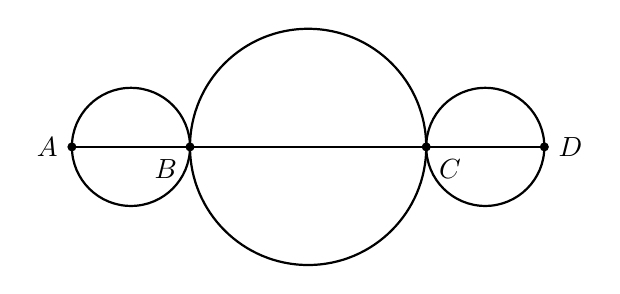
\begin{tikzpicture} [
    point/.style = {draw, circle, fill = black, inner sep = 1pt}
]

% points and segment
\node (A) at (-3, 0) [point, label = left:$A$] {};
\node (B) at (-1.5, 0) [point, label = below left:$B$] {};
\node (C) at (1.5, 0) [point, label = below right:$C$] {};
\node (D) at (3, 0) [point, label = right:$D$] {};
\draw [thick] (A) -- (D);

% circles
\draw [thick] (0,0) circle (1.5);
\draw [thick] (-4.5/2,0) circle (1.5/2);
\draw [thick] (4.5/2,0) circle (1.5/2);

\end{tikzpicture}
\end{document}


%%% opt-q2.png
\documentclass[border=1mm,10pt]{standalone}
\usepackage[utf8]{inputenc}
\usepackage{tikz}
\usepackage{tikz-layers}
\usetikzlibrary{shapes.geometric}
\usetikzlibrary{calc}

% right angles
\def\ralen{.7em}
\newcommand{\drawRightAngle}[3] {
    \draw let \p1 = ($#2!\ralen!#1$),
        \p2 = ($#2!\ralen!#3$),
        \p3 = ($(\p1)+(\p2)-#2$)
    in
        (\p1) -- (\p3) -- (\p2);
}

% background colors
\definecolor{bg1}{RGB}{255,255,248} % fffff8
\definecolor{bg2}{RGB}{243,243,230} % f3f3e6

\begin{document}
\begin{tikzpicture} [
    scale = 1,
    point/.style = {draw, circle, fill = black, inner sep = 1pt}
]

% triangle
\node (A) at (0, 3) [point, label = above:$A$] {};
\node (B) at (0, 0) [point, label = below left:$B$] {};
\node (C) at (6, 0) [point, label = right:$C$] {};
\draw [thick] (A) -- (B) -- (C) -- (A);
\drawRightAngle{(A)}{(B)}{(C)}

% P and Q
\node (P) at (0, 1.2) [red, draw, circle, fill=red, inner sep=1pt, label=above right:$\color{red} P$] {};
\node (Q) at (3.6, 0) [red, draw, circle, fill=red, inner sep=1pt, label=above:$\color{red} Q$] {};
\draw [red, thick] (P) -- (Q);

% lengths
\def\lsep{0.2}
\begin{scope}[on behind layer]
    \draw [dashed, out=-110, in=110] (A) to node [fill=bg2] {5} (B);
    \draw [dashed, out=-15, in=195] (B) to node [fill=bg2] {10} (C);
    \draw [red, dashed, out=-60, in=60] (P) to node [fill=bg2] {$t$} (B);
    \draw [red, dashed, out=20, in=160] (Q) to node [fill=bg2] {$2t$} (C);
    \draw [red, dashed, out=5, in=140] (P) to node [fill=bg2] {$d(t)$} (Q);
\end{scope}

\end{tikzpicture}

\end{document}